%---------------------------------------------------------------------
%
%                          Ap�ndice 1
%
%---------------------------------------------------------------------

\chapter{Secuencia de intercambio de mensajes}
\ref{ap:IntercambioMensajes}


%-------------------------------------------------------------------


\begin{figure}[h!]
	\centering
	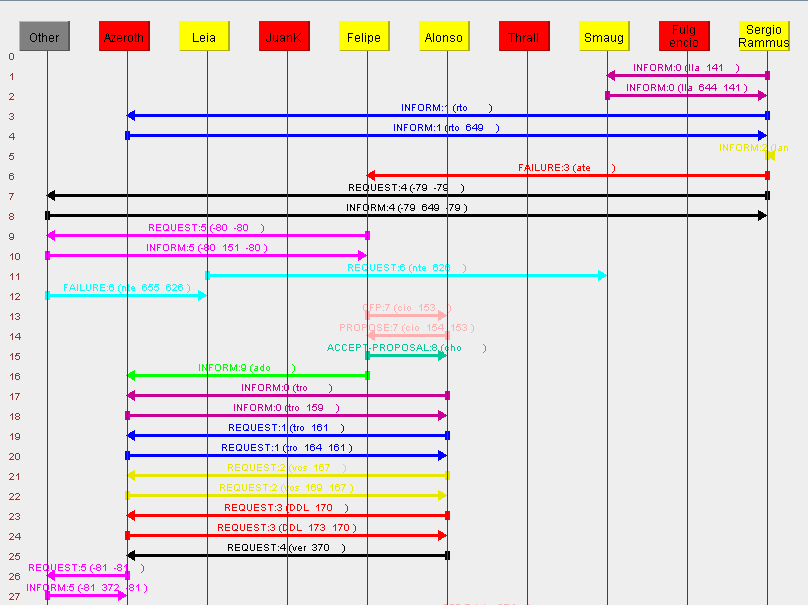
\includegraphics[width=1\textwidth]{Imagenes/EjemploSniffer1}
	\caption{Diagrama de ejemplo de intercambio de mensajes 1}
	\label{fig:EjemploSniffer1}
\end{figure}

\newpage

\begin{lstlisting}[basicstyle=\scriptsize,frame=trBL,caption={Extracto secuencia mensajes FIPA},label=secuenciaMnsjsFIPA]

(INFORM
:sender  ( agent-identifier :name Smaug@147.96.125.224:1099/JADE  
:addresses (sequence http://TheRoad:7778/acc ))
:receiver  (set ( agent-identifier 
	:name SergioRammus@147.96.125.224:1099/JADE  
	:addresses (sequence http://TheRoad:7778/acc )) )
:content  "110" 
:reply-with  SergioRammus@147.96.125.224:1099/JADE1472472185644  
:in-reply-to  batalla1472472185141  :conversation-id  Batalla )
(INFORM
:sender  ( agent-identifier :name SergioRammus@147.96.125.224:1099/JADE  :addresses (sequence http://TheRoad:7778/acc ))
:receiver  (set ( agent-identifier 
	:name Azeroth@147.96.125.224:1099/JADE  
	:addresses (sequence http://TheRoad:7778/acc )) )
:content  "SergioRammus" 
:conversation-id  Muerto )
(INFORM
:sender  ( agent-identifier :name Azeroth@147.96.125.224:1099/JADE  
	:addresses (sequence http://TheRoad:7778/acc ))
:receiver  (set ( agent-identifier 
	:name SergioRammus@147.96.125.224:1099/JADE  
	:addresses (sequence http://TheRoad:7778/acc )) )
:reply-with  SergioRammus@147.96.125.224:1099/JADE1472472185649  
	:conversation-id  Muerto )
(INFORM
:sender  ( agent-identifier :name SergioRammus@147.96.125.224:1099/JADE  :addresses (sequence http://TheRoad:7778/acc ))
:receiver  (set ( agent-identifier 
	:name SergioRammus@147.96.125.224:1099/JADE  
	:addresses (sequence http://TheRoad:7778/acc )) )
:conversation-id  Fin-Plan )
(FAILURE
:sender  ( agent-identifier :name SergioRammus@147.96.125.224:1099/JADE  :addresses (sequence http://TheRoad:7778/acc ))
:receiver  (set ( agent-identifier 
	:name Felipe@147.96.125.224:1099/JADE  
	:addresses (sequence http://TheRoad:7778/acc )) )
:conversation-id  Rescate )
(REQUEST
:sender  ( agent-identifier :name SergioRammus@147.96.125.224:1099/JADE  :addresses (sequence http://TheRoad:7778/acc ))
:receiver  (set ( agent-identifier :name df@147.96.125.224:1099/JADE  
	:addresses (sequence http://TheRoad:7778/acc )) )
:content  "((action ( agent-identifier 
	:name df@147.96.125.224:1099/JADE  
	:addresses (sequence http://TheRoad:7778/acc ))
		(deregister (df-agent-description :name ( agent-identifier 
		:name SergioRammus@147.96.125.224:1099/JADE  
		:addresses (sequence http://TheRoad:7778/acc ))))))" 
:reply-with  rw-SergioRammus@147.96.125.224:1099/JADE1472472186648-79  :language  fipa-sl0  :ontology  FIPA-Agent-Management  
	:protocol  fipa-request
:conversation-id  
	conv-SergioRammus@147.96.125.224:1099/JADE1472472186648-79 )

\end{lstlisting}

\begin{figure}[h]
	\centering
	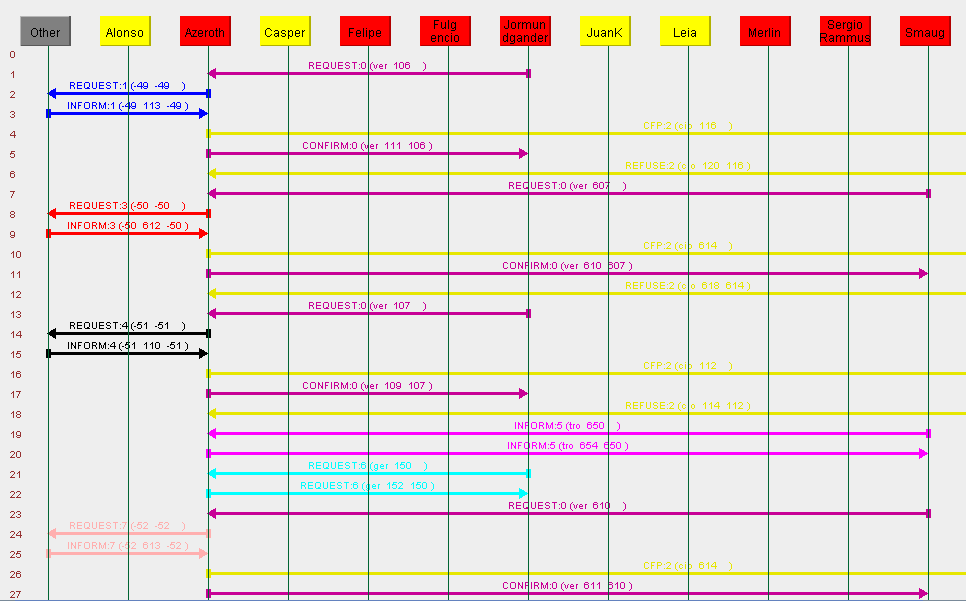
\includegraphics[width=0.9\textwidth]{Imagenes/EjemploSniffer2}
	\caption{Diagrama de ejemplo de intercambio de mensajes 2}
	\label{fig:EjemploSniffer2}
\end{figure}


